\documentclass{article}
\usepackage{graphicx} % Required for inserting images
\usepackage{amsmath}
\usepackage[english, russian] {babel}
\usepackage[utf8]{inputenc}
\usepackage[T2A]{fontenc}
\usepackage{minted}
\usepackage{float}
\usepackage{amssymb}
\usepackage{mathtools}

\title{Дефференцальные уравнения. Лекции}
\author{silvia.lesnaia }
\date{February 2025}

\begin{document}

\maketitle

\textbf{21.02.25}

\section{Элементы комбинаторики}

\subsection{Основные правила комбинаторики}


\textbf{Правило произдведения}

ПП A-m B-n $\implies$ (A,B) - mn

\textbf{Правило суммы}

П$\Sigma$ A-m B-n $\implies$ (A,B) - A(m) + B(n)
\vspace{5mm}

\textbf{Размещение} 

$\bar{A}_{n}^{k} = n^k$ с повторерениям

$A_{n}^{k} = \frac{n!}{(n-k)!} = n(n-1)... (n_k+1)$ без повторерений


\vspace{5mm}
\textbf{Перестоновки} 

Перестоновка без повторерени $P_n=n!$

Перестоновка с повторерениям $\bar{P}_n = \frac{n!}{n_1!n_2!...n_k}$


\vspace{5mm}
\textbf{Сочетания}

Без повторерения $C_{n}^{k} = \frac{n!}{k!(n-k)!}$

k!$C_{n}^{k}=A_{n}^{k}$

\vspace{1cm}

Биноминальный свойства 

1. $C_{n}^{k} = \bar{P}(k<n-k)$

2. Свойства симметричности $C_{n}^{k} = C_{n}^{n-k}$

3. Основаное свойство  $C_{n}^{k} = C_{n-1}^{k-1} + C_{n-1}^{k}$

4. Суммы сочетания  $C_{n}^{0} + C_{n-}^{1} + C_{n}^{2}+...+C_{n}^{n}=2^n$

5. Знак переменной суммы сочетания 
$C_{n}^{0} - C_{n-}^{1} + C_{n}^{2}-...+(-1)C_{n}^{n} = 0$

\vspace{5mm}

С повторерениям 

$\bar{C_{n}^{0}} = C_{n+k-1}^{k} = \bar{P}(k,n-1)$


\textbf{Формула включения исключения}

$A \neq \varnothing A_1, A_2,...A_n \subseteq A$

\begin{figure}[H]
    \centering
    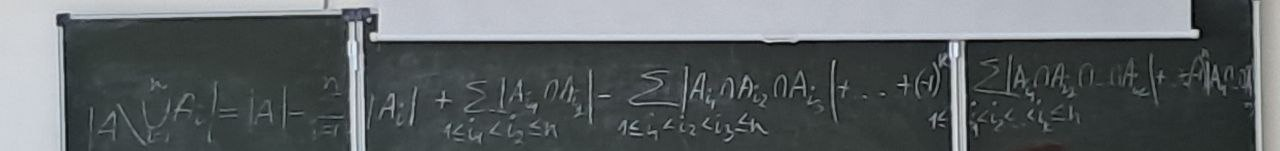
\includegraphics[width=1\linewidth]
    {12c36b33-baa5-41a2-b016-b02e7ad225c8.jpg}
\end{figure}

Докозательство:

\begin{figure}[H]
    \centering
    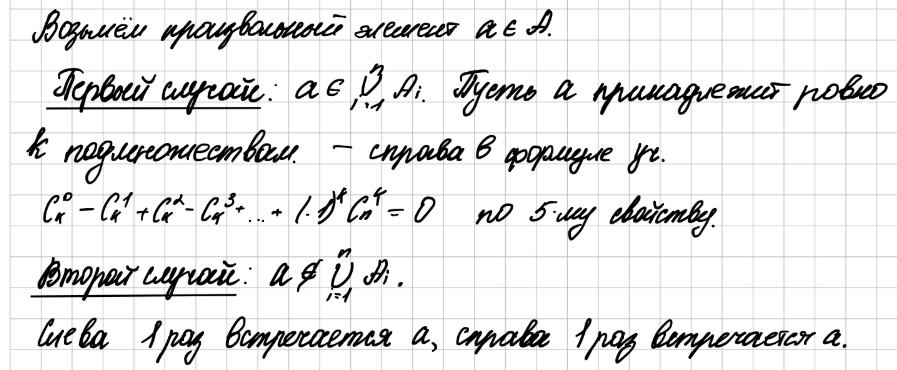
\includegraphics[width=1\linewidth]{Снимок экрана 2025-02-21 145919.png}
\end{figure}

Пример:

$X=\left\{a_1,...,a_n \right\}$

$Y=\left\{b_1,...,b_n\right\}$


\begin{figure}[H]
    \centering
    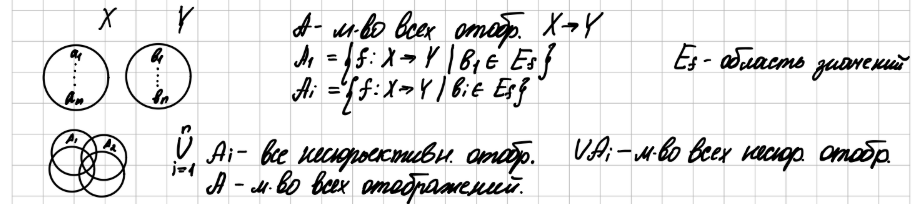
\includegraphics[width=1\linewidth]{Снимок экрана 2025-02-21 150506.png}
\end{figure}

||

||

||


\textbf{07.03.25}
\section{Комбинаторики разбиения}

\textbf{14.04.25}


\section{Графы}





\end{document}